\documentclass[../../main.tex]{subfiles}
\begin{document}

\subsection*{4.1}
Due sfere conduttrici $S_1$ e $S_2$ di raggi $R_1$ e $R_2$ sono poste nel vuoto ad una distanza x tra i centri molto grande rispetto a $R_1$ e $R_2$.
\\La sfera $S_1$, isolata, ha una carica $q_1$ e la sfera $S_2$ è mantenuta al potenziale $V_a$ rispetto all'infinito.
\\Calcolare il potenziale $V_1(x)$ della sfera $S_1$, la carica $q_2(x)$ della sfera $S_2$ e la forza F(x) tra le sfere in funzione della distanza x.
\\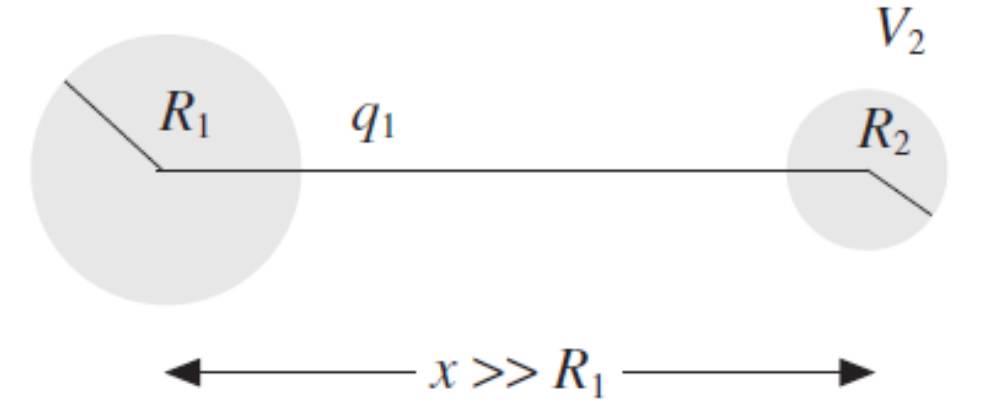
\includegraphics[scale=0.3]{e_4_1.png}
\subsubsection*{Formule utilizzate}
$\sum_i\frac{q_i}{4\pi\epsilon_0r_i}$
\subsubsection*{Soluzione punto a}
Sfera $S_1$
\\$V_1(x) = \frac{1}{4\pi\epsilon_0}\left(\frac{q_1}{R_1}+\frac{q_2(x)}{x}\right)$
\\\\Sfera $S_2$
\\$V_2(x) = \frac{1}{4\pi\epsilon_0}\left(\frac{q_2}{R_2}+\frac{q_1(x)}{x}\right)$
\\Da cui: $q_2(x) = R_2(4\pi\epsilon_0V_2 - \frac{q_1}{x})$
\\Per cui: $V_1(x) = \frac{q_1}{4\pi\epsilon_0}\left(\frac{1}{R_1}-\frac{R_2}{x_2}\right) + \frac{R_2V_2}{x}$
\\Forza: $F(x) = \frac{1}{4\pi\epsilon_0}\frac{q_1q_2(x)}{x^2}$
\\usando $q_2 = ...$
\\$F(x) = \frac{1}{4\pi\epsilon_0}\frac{q_1}{x^2}R_2\left(4\pi\epsilon_0V_2-\frac{q_1}{x}\right)$
\subsubsection*{Soluzione punto b}
\newpage

\end{document}